\documentclass[11pt,a4paper]{article}

\usepackage[margin=2.0cm]{geometry}
\usepackage{amsmath,amssymb}
\usepackage{booktabs}
\usepackage{array}
\usepackage{algorithm}
\usepackage{algpseudocode}
\usepackage{tikz}
\usetikzlibrary{arrows.meta,positioning,calc,fit,backgrounds,shapes.geometric}

\title{MotoMap Algoritma Mantigi\\\large TikZ Node Figure + Matematik + Dijkstra}
\author{MotoMap}
\date{\today}

\begin{document}
\maketitle

\section{Hizli Okuma Haritasi}
Ama\c{c}: motosiklet i\c{c}in yol a\u{g}\i{}n\i{} \emph{feature} seviyesinde zenginle\c{s}tirip,
mod-bazli agirliklarla en uygun rotayi bulmak.

\begin{center}
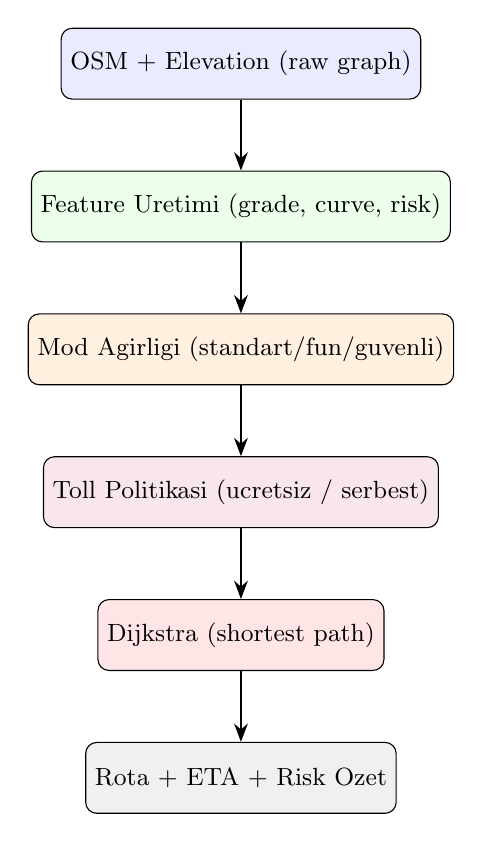
\begin{tikzpicture}[
  box/.style={draw,rounded corners,minimum width=3.4cm,minimum height=9mm,align=center,font=\small},
  arr/.style={-Stealth,thick},
  node distance=9mm
]
\node[box,fill=blue!8] (a) {OSM + Elevation\ \small(raw graph)};
\node[box,fill=green!8,below=of a] (b) {Feature Uretimi\ \small(grade, curve, risk)};
\node[box,fill=orange!12,below=of b] (c) {Mod Agirligi\ \small(standart/fun/guvenli)};
\node[box,fill=purple!10,below=of c] (d) {Toll Politikasi\ \small(ucretsiz / serbest)};
\node[box,fill=red!10,below=of d] (e) {Dijkstra\ \small(shortest path)};
\node[box,fill=gray!12,below=of e] (f) {Rota + ETA + Risk Ozet};

\draw[arr] (a)--(b);
\draw[arr] (b)--(c);
\draw[arr] (c)--(d);
\draw[arr] (d)--(e);
\draw[arr] (e)--(f);
\end{tikzpicture}
\end{center}

\section{Graf ve Feature Modeli}
Yol a\u{g}\i{} yonlu agirlikli graf:
\begin{equation}
G=(V,E), \quad E \subseteq V\times V.
\end{equation}

Kenar ozellikleri:
\begin{equation}
\mathbf{x}_e = [L_e, v^{max}_e, grade_e, curve_e, risk_e, toll_e, road\_type_e].
\end{equation}

\subsection{Temel sure}
\begin{equation}
T_e = \frac{L_e}{\max\left(1,\frac{v^{max}_e\cdot\phi}{3.6}\right)} + \delta,
\end{equation}
\(\phi=\texttt{MOTOMAP\_SPEED\_FACTOR},\;\delta=\texttt{MOTOMAP\_SEGMENT\_DELAY\_S}\).

\subsection{Viraj ve risk}
\begin{align}
N_{fun}(e)&=\#\{\theta:15^\circ<\theta<45^\circ\},\\
N_{danger}(e)&=\#\{\theta:\theta>60^\circ\},\\
S_{curve}(e)&=\frac{N_{fun}(e)}{1+N_{danger}(e)},\\
risk_e&=\mathbb{I}[hairpin(e)>0\land grade_e<-0.08].
\end{align}

\begin{center}
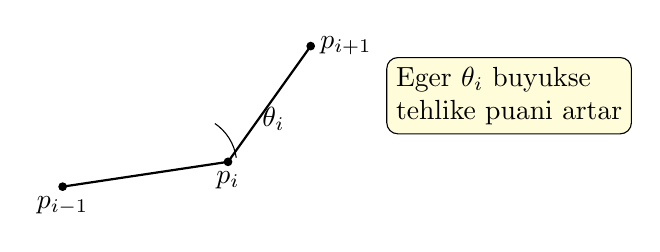
\begin{tikzpicture}[>=Stealth,scale=1.05]
\coordinate (p1) at (0,0);
\coordinate (p2) at (2,0.3);
\coordinate (p3) at (3.0,1.7);
\draw[thick] (p1)--(p2)--(p3);
\fill (p1) circle (1.5pt) node[below] {$p_{i-1}$};
\fill (p2) circle (1.5pt) node[below] {$p_i$};
\fill (p3) circle (1.5pt) node[right] {$p_{i+1}$};
\draw (2.1,0.35) arc[start angle=8,end angle=56,radius=0.6];
\node at (2.55,0.82) {$\theta_i$};
\node[draw,rounded corners,fill=yellow!15,align=left] at (5.4,1.1)
{Eger $\theta_i$ buyukse\\tehlike puani artar};
\end{tikzpicture}
\end{center}

\section{Mod Bazli Maliyet Fonksiyonlari}
\subsection{Standart}
\begin{equation}
W^{std}_e = T_e\,(1+p_{road}(e)).
\end{equation}

\subsection{Viraj keyfi}
\begin{align}
B_e &= 1 + 0.55S_{curve}(e) + 0.14N_{fun}(e) + b_{road}(e),\\
P_e &= 1 + 0.12N_{danger}(e) + 0.45risk_e,\\
W^{fun}_e &= \frac{T_e}{\max(10^{-6},B_e)}\,P_e.
\end{align}

\subsection{Guvenli}
\begin{align}
d_e &= \max(0,|\min(0,grade_e)|-0.08),\\
P^{safe}_e &= 1 + 0.55N_{danger}(e)+1.40risk_e+5.00d_e+p^{safe}_{road}(e),\\
W^{safe}_e &= T_e\,P^{safe}_e.
\end{align}

\section{Algoritmalar (Adim Adim)}

\subsection{Algoritma-1: Feature graph olusturma}
\begin{algorithm}[h]
\caption{BuildFeatureGraph}
\begin{algorithmic}[1]
\Require Raw graph $G$
\State $G \leftarrow$ legal olmayan kenarlari filtrele
\State node elevation ekle, edge grade hesapla
\State eksik lanes/maxspeed/surface alanlarini doldur
\State viraj acilarindan $N_{fun},N_{danger},S_{curve}$ cikar
\State her edge icin $risk_e$ isaretle
\State \Return $G$
\end{algorithmic}
\end{algorithm}

\subsection{Algoritma-2: Mod bazli kenar agirligi}
\begin{algorithm}[h]
\caption{ComputeWeightByMode}
\begin{algorithmic}[1]
\Require edge $e$, mode $m \in \{std,fun,safe\}$
\State taban sure $T_e$ hesapla
\If{$m=std$}
  \State \Return $W^{std}_e$
\ElsIf{$m=fun$}
  \State \Return $W^{fun}_e$
\Else
  \State \Return $W^{safe}_e$
\EndIf
\end{algorithmic}
\end{algorithm}

\subsection{Algoritma-3: Ucretli/Ucretsiz secim}
\begin{algorithm}[h]
\caption{SelectRouteWithTollPreference}
\begin{algorithmic}[1]
\Require source $s$, target $t$, preference $p$
\State $\pi_{serbest} \leftarrow \text{Dijkstra}(G,s,t)$
\State $\pi_{ucretsiz} \leftarrow \text{Dijkstra}(G\setminus E_{toll},s,t)$
\If{$p=\texttt{ucretsiz}$}
  \State \Return $\pi_{ucretsiz}$
\Else
  \State \Return $\pi_{serbest}$
\EndIf
\end{algorithmic}
\end{algorithm}

\subsection{Algoritma-4: Dijkstra cekirdegi}
\begin{algorithm}[h]
\caption{Dijkstra}
\begin{algorithmic}[1]
\Require $G=(V,E)$, $s$, $t$, positive edge weights
\State $dist[v]\gets\infty$, $dist[s]\gets 0$
\State priority queue $Q\gets\{(0,s)\}$
\While{$Q$ not empty}
  \State extract $(d,u)$ with min key
  \If{$u=t$} \State \textbf{break} \EndIf
  \For{each edge $(u,v)$}
    \State $alt\gets d+W_{uv}$
    \If{$alt<dist[v]$}
      \State update $dist[v], parent[v]$
      \State push $(alt,v)$
    \EndIf
  \EndFor
\EndWhile
\State reconstruct path using $parent$
\end{algorithmic}
\end{algorithm}

\section{TikZ ile Hemen Anlasilir Ornekler}

\subsection{Modlarin ayni graf uzerinde farkli rota secmesi}
\begin{center}
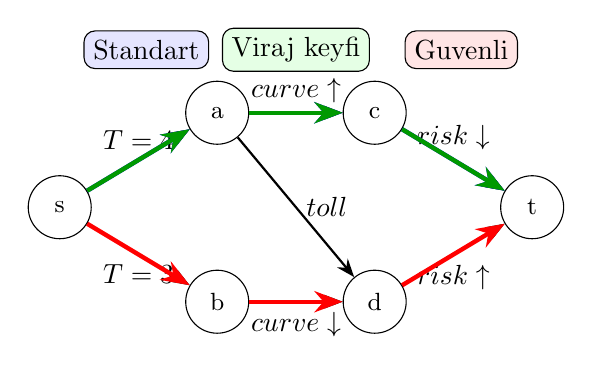
\begin{tikzpicture}[
  >=Stealth,
  vtx/.style={circle,draw,minimum size=8mm,font=\small},
  e/.style={->,thick}
]
\node[vtx] (s) at (0,0) {s};
\node[vtx] (a) at (2,1.2) {a};
\node[vtx] (b) at (2,-1.2) {b};
\node[vtx] (c) at (4,1.2) {c};
\node[vtx] (d) at (4,-1.2) {d};
\node[vtx] (t) at (6,0) {t};

\draw[e] (s)--(a) node[midway,above] {$T=4$};
\draw[e] (a)--(c) node[midway,above] {$curve\uparrow$};
\draw[e] (c)--(t) node[midway,above] {$risk\downarrow$};

\draw[e] (s)--(b) node[midway,below] {$T=3$};
\draw[e] (b)--(d) node[midway,below] {$curve\downarrow$};
\draw[e] (d)--(t) node[midway,below] {$risk\uparrow$};

\draw[e] (a)--(d) node[midway,right] {$toll$};

\draw[ultra thick,blue,->] (s)--(a);
\draw[ultra thick,blue,->] (a)--(c);
\draw[ultra thick,blue,->] (c)--(t);

\draw[ultra thick,green!60!black,->] (s)--(a);
\draw[ultra thick,green!60!black,->] (a)--(c);
\draw[ultra thick,green!60!black,->] (c)--(t);

\draw[ultra thick,red,->] (s)--(b);
\draw[ultra thick,red,->] (b)--(d);
\draw[ultra thick,red,->] (d)--(t);

\node[draw,rounded corners,fill=blue!10] at (1.1,2.0) {Standart};
\node[draw,rounded corners,fill=green!10] at (3.0,2.0) {Viraj keyfi};
\node[draw,rounded corners,fill=red!10] at (5.1,2.0) {Guvenli};
\end{tikzpicture}
\end{center}

\subsection{Dijkstra queue evrimi (node-state gorunumu)}
\begin{center}
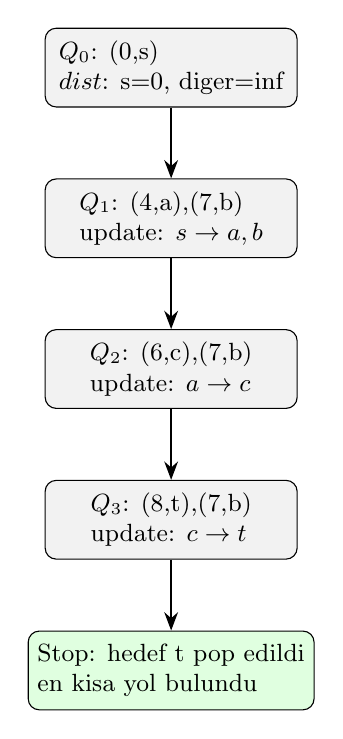
\begin{tikzpicture}[
  box/.style={draw,rounded corners,minimum width=3.2cm,minimum height=10mm,align=left,font=\small},
  arr/.style={-Stealth,thick},
  node distance=9mm
]
\node[box,fill=gray!10] (q0) {$Q_0$: (0,s)\\$dist$: s=0, diger=inf};
\node[box,fill=gray!10,below=of q0] (q1) {$Q_1$: (4,a),(7,b)\\update: $s\to a,b$};
\node[box,fill=gray!10,below=of q1] (q2) {$Q_2$: (6,c),(7,b)\\update: $a\to c$};
\node[box,fill=gray!10,below=of q2] (q3) {$Q_3$: (8,t),(7,b)\\update: $c\to t$};
\node[box,fill=green!12,below=of q3] (q4) {Stop: hedef t pop edildi\\en kisa yol bulundu};
\draw[arr] (q0)--(q1);
\draw[arr] (q1)--(q2);
\draw[arr] (q2)--(q3);
\draw[arr] (q3)--(q4);
\end{tikzpicture}
\end{center}

\subsection{Toll filtre etkisi}
\begin{center}
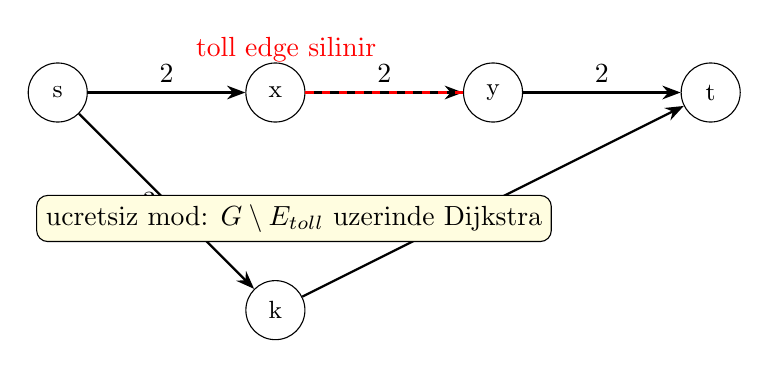
\begin{tikzpicture}[>=Stealth, node distance=2cm,
  vtx/.style={circle,draw,minimum size=7.5mm,font=\small},
  e/.style={->,thick},
  rm/.style={red,dashed,thick}]

\node[vtx] (s) {s};
\node[vtx,right=of s] (x) {x};
\node[vtx,right=of x] (y) {y};
\node[vtx,right=of y] (t) {t};
\node[vtx,below=of x] (k) {k};

\draw[e] (s)--(x) node[midway,above] {$2$};
\draw[e] (x)--(y) node[midway,above] {$2$};
\draw[e] (y)--(t) node[midway,above] {$2$};
\draw[e] (s)--(k) node[midway,left] {$3$};
\draw[e] (k)--(t) node[midway,below] {$6$};

\draw[rm] (x)--(y);
\node[red] at (2.9,0.55) {toll edge silinir};
\node[draw,rounded corners,fill=yellow!12] at (3.0,-1.6)
{ucretsiz mod: $G\setminus E_{toll}$ uzerinde Dijkstra};
\end{tikzpicture}
\end{center}

\section{Dogruluk ve Karmasiklik}
\begin{itemize}
  \item Tum kenar agirliklari pozitif oldugunda Dijkstra optimal sonucu verir.
  \item Binary heap ile karmasiklik:
  \begin{equation}
  \mathcal{O}((|V|+|E|)\log|V|).
  \end{equation}
  \item Bu nedenle maliyet fonksiyonunda negatif agirlik uretmemek kritik tasarim kosuludur.
\end{itemize}

\section{Semboller}
\begin{center}
\begin{tabular}{@{}ll@{}}
\toprule
Sembol & Anlam \\
\midrule
$L_e$ & Kenar uzunlugu (m) \\
$v^{max}_e$ & Kenar speed limit (km/h) \\
$T_e$ & Taban gecis suresi \\
$N_{fun},N_{danger}$ & Viraj sayaclari \\
$S_{curve}$ & Viraj keyfi skoru \\
$risk_e$ & Yuksek risk indikatoru \\
$W_e$ & Nihai kenar agirligi \\
\bottomrule
\end{tabular}
\end{center}

\end{document}
